\documentclass[border=10pt]{standalone}

\usepackage{tikz}
\usepackage{tikzsymbols}
\usetikzlibrary{calc,patterns,shapes.geometric}

\def\centerarc[#1](#2)(#3:#4:#5){\draw[#1] ($(#2)+({#5*cos(#3)},{#5*sin(#3)})$) arc (#3:#4:#5);}

\begin{document}
	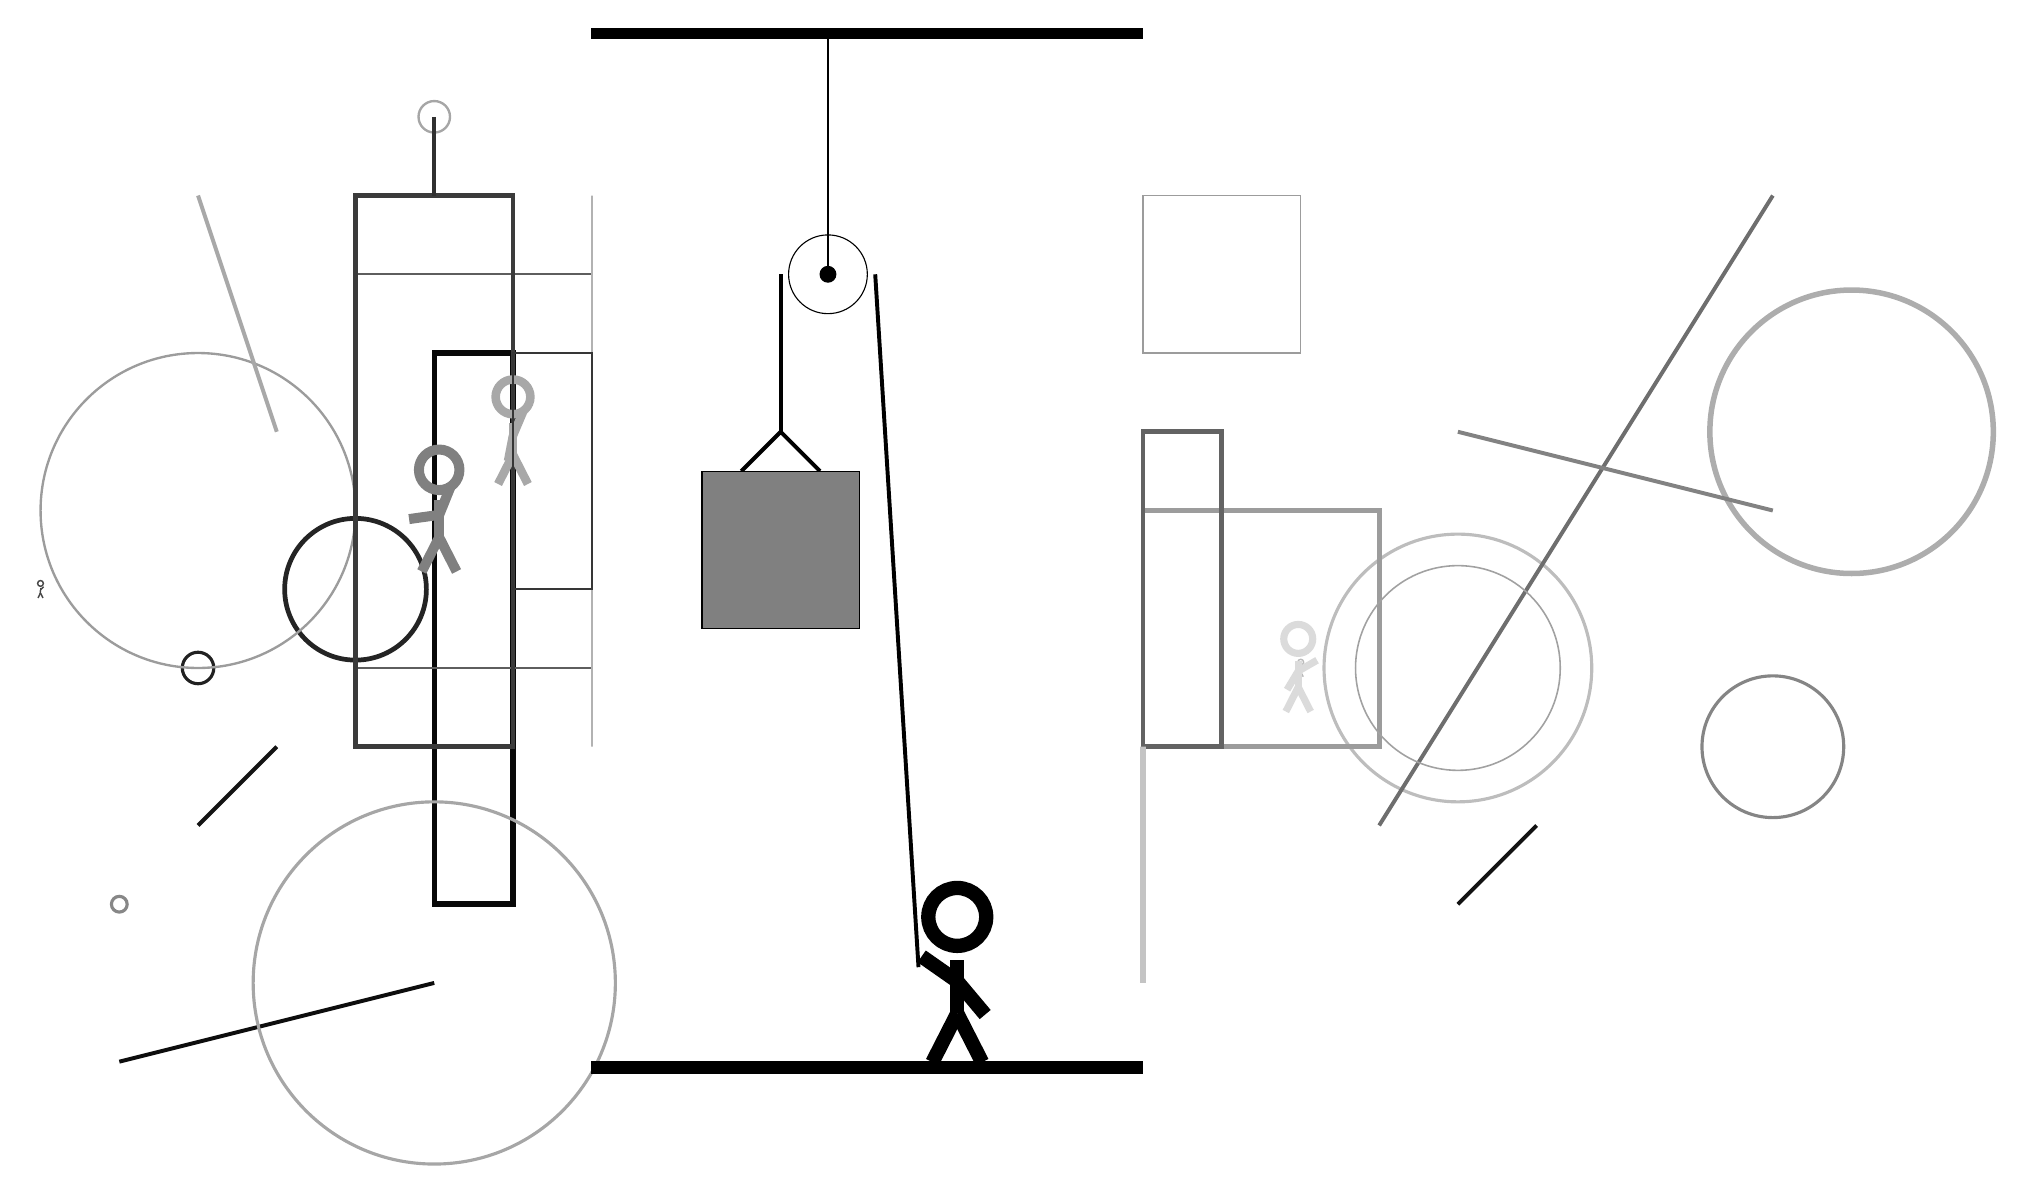
\begin{tikzpicture}
		%%%%% START %%%%%
		
		\draw[fill=black] (-2, 10) rectangle (5, 10.125);
		
		\draw[line width=0.5mm, color=black!93](9, -1) -- (10, 0);
		
		\node[line width=0.4mm, color=black!27] at (7, 2) {\Strichmaxerl[1][36][64]};
		\draw [line width=0.4mm, color=black!26](9, 2) circle (1.7);
		\node[line width=0.4mm, color=black!72] at (-9, 3) {\Strichmaxerl[1][85][46]};
		\draw[line width=0.5mm, color=black!95](-4, -2) -- (-8, -3);
		\draw[line width=0.7mm, color=black!97] (-3, -1) rectangle (-4, 6);
		
		\draw [line width=0.4mm, color=black!87](-7, 2) circle (0.2);
		\draw [line width=0.4mm, color=black!35](-4, -2) circle (2.3);
		\draw [line width=0.4mm, color=black!47](-8, -1) circle (0.1);
		\draw [line width=0.6mm, color=black!86](-5, 3) circle (0.9);
		
		\draw [line width=0.3mm, color=black!39](-7, 4) circle (2.0);
		
		\node[line width=0.7mm, color=black!50] at (-4, 4) {\Strichmaxerl[7][8][68]};
		\draw[line width=0.6mm, color=black!39] (5, 1) rectangle (8, 4);
		
		\draw [line width=0.7mm, color=black!32](14, 5) circle (1.8);
		\draw[line width=0.2mm, color=black!63] (-2, 7) rectangle (-5, 2);
		\draw[line width=0.6mm, color=black!77] (-3, 8) rectangle (-5, 1);
		
		\draw[line width=0.6mm, color=black!61] (5, 5) rectangle (6, 1);
		\draw[line width=0.2mm, color=black!39] (7, 8) rectangle (5, 6);
		\draw[line width=0.5mm, color=black!34](-7, 8) -- (-6, 5);
		\draw [line width=0.4mm, color=black!48](13, 1) circle (0.9);
		\node[line width=0.6mm, color=black!34] at (-3, 5) {\Strichmaxerl[6][79][67]};
		
		\draw[line width=0.7mm, color=black!23] (5, 1) rectangle (5, -2);
		
		\draw[line width=0.2mm, color=black!30] (-2, 8) rectangle (-2, 1);
		\draw [line width=0.3mm, color=black!35](-4, 9) circle (0.2);
		\draw[line width=0.5mm, color=black!81](-4, 9) -- (-4, 8);
		
		\draw[line width=0.3mm, color=black!79] (-2, 6) rectangle (-3, 3);
		\draw[line width=0.5mm, color=black!57](8, 0) -- (13, 8);
		\draw [line width=0.2mm, color=black!37](9, 2) circle (1.3);
		
		\node[line width=0.3mm, color=black!14] at (7, 2) {\Strichmaxerl[5][59][30]};
		
		\draw[line width=0.5mm, color=black!92](-7, 0) -- (-6, 1);
		\draw[line width=0.5mm, color=black!49](9, 5) -- (13, 4);
		
		
		\draw (1, 7) circle (0.5);
		\draw[fill=black] (1, 7) circle (0.1);
		\draw (1, 10) -- (1, 7);
		
		\draw[line width=0.5mm] (-0.1, 4.5) -- (0.4, 5.0) -- (0.9, 4.5);
		\draw[fill=black!50] (-0.6, 4.5) rectangle (1.4, 2.5);
		
		\draw[line width=0.5mm] (0.4, 7) -- (0.4, 5.0);
		\centerarc[line width=0.5mm](1, 7)(0:180:0.6);
		\draw[line width=0.5mm](1.6, 7) -- (2.15, -1.8);
		
		\node at (2.6, -1.9) {\Strichmaxerl[10][-35][-50]};
		
		\draw[fill=black] (-2, -3) rectangle (5, -3.15);
		
		%%%%% END %%%%%
	\end{tikzpicture}
\end{document}